\section{Experiments}
\subsection{Experiment Setups}\label{sec_expsetup}
In addition to the synthetic experiment, we evaluate BARL on math tasks. We implement BARL across various models, including Qwen2.5-Math-1.5B, Qwen2.5-Math-7B \citep{yang2024qwen25mathtechnicalreportmathematical}, and DeepSeek-R1-Distill-Llama-8B \citep{guo2025deepseek}. Training is conducted on the Big-Math dataset \citep{albalak2025big}, and evaluation is performed on four benchmarks: GSM8K \citep{cobbe2021training}, MATH \citep{hendrycks2021measuring}, CollegeMath \citep{tang2024mathscale}, and OlympiadBench \citep{he2024olympiadbench}. During training, the maximum prompt length is set to $512$ and the maximum response length is set to $1024$. For BARL, we set $\beta=1$ and $|\mathcal{M}|=5$ in Algorithm \ref{algorithm}.

We compare BARL against two RL baselines that span outcome- and process-reward RL. For the outcome-reward GRPO baseline, we set its group size to $5$ for a fair comparison with BARL and, after performing a grid search over the KL‐divergence coefficients $[0, 0.001, 0.005, 0.01]$, adopt $0.005$ as it yields the best overall performance across all benchmarks. For the process-reward baseline, we adapt a variant of MRT \citep{qu2025optimizing} by integrating the progress reward defined in \eqref{def_r} into the outcome reward, which we refer to as \textit{progress} in the following sections. For all algorithms, we set the training and rollout batch sizes to $128$ and $1024$, respectively. We train the Qwen and Llama models for $110$ and $60$ iterations, respectively, defined w.r.t. the rollout batches. The temperature during online sampling is $1.0$ and is $0.0$ during evaluation. For both BARL and the progress baseline, we set the number of tokens for each reasoning step as $128$.

\subsection{Experiment Results}
We report the pass@1 accuracies in Table \ref{tab_perf}. All models are trained using three random seeds, and we calculate the mean and standard error of the resulting accuracies. For each algorithm, we report the results of the checkpoint that has the overall best performance on all benchmarks. 

\begin{table*}[ht]
\small
\vspace{-0.1cm}
\centering
\begin{tabular}{l|ccccccc}
\hline
Model     & GSM8K & MATH & College & Olympiad & AIME & AMC & Average \\ \hline
Qwen-1.5B  & $40.0$ & $34.1$ & $6.6$ & $21.8$ & 16.7 & 32.5 & $25.3$  \\
\quad GRPO  & $83.9\scriptstyle(\pm0.5)$ & $71.5\scriptstyle(\pm0.4)$ & $45.1\scriptstyle(\pm0.3)$ & $31.6\scriptstyle(\pm0.4)$ & $\textbf{17.8}\scriptstyle(\pm0.9)$  & $55.8\scriptstyle(\pm0.7)$ & $51.0\scriptstyle(\pm0.3)$  \\
\quad Progress  & $84.8\scriptstyle(\pm0.6)$ & $72.1\scriptstyle(\pm0.4)$ & $45.9\scriptstyle(\pm0.3)$ & $35.5\scriptstyle(\pm0.3)$ & $14.4\scriptstyle(\pm0.9)$ & $55.8\scriptstyle(\pm0.7)$ & $51.4\scriptstyle(\pm0.2)$ \\
\quad BARL  & $\textbf{85.8}\scriptstyle(\pm0.1)$ & $\textbf{72.7}\scriptstyle(\pm0.3)$ & $\textbf{46.8}\scriptstyle(\pm0.2)$ & $\textbf{35.8}\scriptstyle(\pm0.3)$ &  $\textbf{17.8}\scriptstyle(\pm0.9)$  & $\textbf{60.8}\scriptstyle(\pm0.7)$ &$\textbf{53.3}\scriptstyle(\pm0.4)$ \\
\hline
Qwen-7B  & 59.1 & 53.7  & 21.9 & 19.0  & 13.3 & 42.5 & 34.9 \\
\quad GRPO  & $90.3\scriptstyle(\pm0.1)$ & $77.6\scriptstyle(\pm0.4)$ & $47.0\scriptstyle(\pm0.3)$ & $38.5\scriptstyle(\pm0.2)$ & $24.5\scriptstyle(\pm0.4)$ & $65.0\scriptstyle(\pm1.2)$ & $57.1\scriptstyle(\pm0.2)$ \\
\quad Progress  & $91.1\scriptstyle(\pm0.3)$ &  $78.8\scriptstyle(\pm0.1)$ & $46.7\scriptstyle(\pm0.1)$ & $41.1\scriptstyle(\pm0.2)$ & $24.5\scriptstyle(\pm0.4)$ &  $65.4\scriptstyle(\pm1.4)$ & $57.9\scriptstyle(\pm0.2)$  \\
\quad BARL & $\textbf{91.7}\scriptstyle(\pm0.2)$ & $\textbf{79.2}\scriptstyle(\pm0.3)$ & $\textbf{47.5}\scriptstyle(\pm0.2)$ & $\textbf{42.0}\scriptstyle(\pm0.4)$ & $\textbf{29.0}\scriptstyle(\pm0.4)$ & $\textbf{66.7}\scriptstyle(\pm1.4)$ &  $\textbf{59.4}\scriptstyle(\pm0.3)$  \\
\hline
Llama-8B  & $82.0$ & $65.7$ & $35.8$ & $26.5$  & $10.0$ & $42.5$ & $43.7$   \\
\quad GRPO  & $85.7\scriptstyle(\pm0.5)$ & $\textbf{74.3}\scriptstyle(\pm0.4)$ & $39.6\scriptstyle(\pm0.3)$ & $36.0\scriptstyle(\pm0.5)$ & $16.7\scriptstyle(\pm0.8)$ & $60.4\scriptstyle(\pm0.3)$ & $52.1\scriptstyle(\pm0.4)$ \\
\quad Progress  & $\textbf{85.9}\scriptstyle(\pm0.4)$ & $73.9\scriptstyle(\pm0.4)$ & $39.8\scriptstyle(\pm0.5)$ & $35.3\scriptstyle(\pm0.2)$ & $15.0\scriptstyle(\pm0.8)$ & $55.8\scriptstyle(\pm0.7)$ & $51.0\scriptstyle(\pm0.4)$\\
\quad BARL  & $85.4\scriptstyle(\pm0.6)$ & $73.9\scriptstyle(\pm0.6)$ & $\textbf{40.4}\scriptstyle(\pm0.3)$ & $\textbf{37.2}\scriptstyle(\pm0.5)$ & $\textbf{17.8}\scriptstyle(\pm0.9)$ & $\textbf{61.7}\scriptstyle(\pm0.7)$ & $\textbf{52.7}\scriptstyle(\pm0.4)$  \\
\hline
\end{tabular}
\caption{Mean and standard error of the accuracies over three independent training runs.}
\label{tab_perf}
\end{table*}

We observe that BARL achieves higher accuracies across most benchmarks and models. It consistently outperforms the two conventional RL baselines in terms of average accuracy, with the most significant gains observed on challenging benchmarks that demand effective exploration. Notably, BARL delivers these gains with minimal computational overhead, which comes from calculating the probabilities of candidate answers at the end of each step, reusing the prefix cache from CoT generations. We defer the curves of accuracies and response lengths to Appendix \ref{app_acc_eval} and \ref{app_len_eval}.

\subsection{Ablation Studies}\label{sec_ablation}
\paragraph{Token Efficiency.} We evaluate the token efficiency of BARL and baseline models by measuring the total number of tokens required to solve a problem. Specifically, in Figure \ref{fig_ablation_token}, we plot the pass@k accuracies and the corresponding average numbers of tokens, serving as a proxy for performance per token. In all the following ablations, we mainly analyze the models fine-tuned from Qwen2.5-Math-1.5B. We vary k from $1$ to $6$ and set the temperature to $1.0$, but observe that the GRPO and base models are less robust under sampling, resulting in decreased pass@1 performance (see Appendix \ref{app_greedy}). To account for this, we combine greedy decoding outputs with sampled outputs when computing token usage and accuracy. 
We omit the base model from the plots due to its significantly higher token consumption and lower asymptotic accuracy. We find that BARL achieves higher accuracies with substantially fewer tokens, requiring up to \textbf{39\%} fewer average tokens than the progress baseline, \textbf{50\%} fewer than GRPO, and over \textbf{90\%} fewer than the base model.
\begin{figure}[h]
\vspace{-0.1cm}
    \centering
    \begin{minipage}[b]{0.245\linewidth}
        \centering
    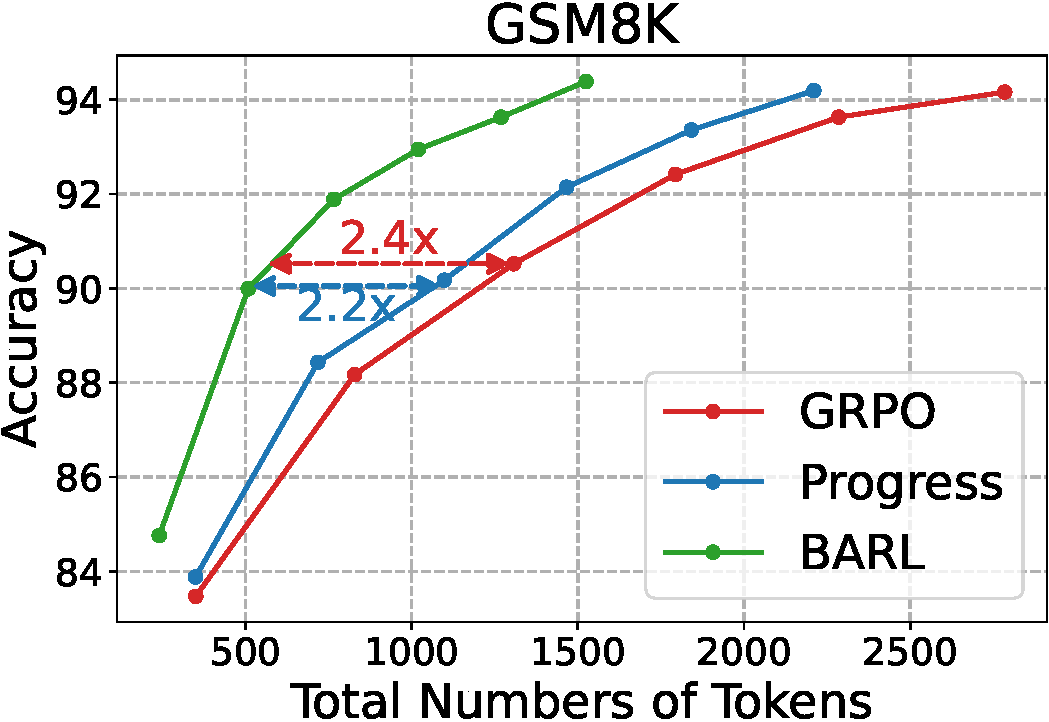
\includegraphics[width=1.005\linewidth]{figs/qwen15_gsm_token_2.pdf}
    \end{minipage}
    \begin{minipage}[b]{0.245\linewidth}
        \centering
        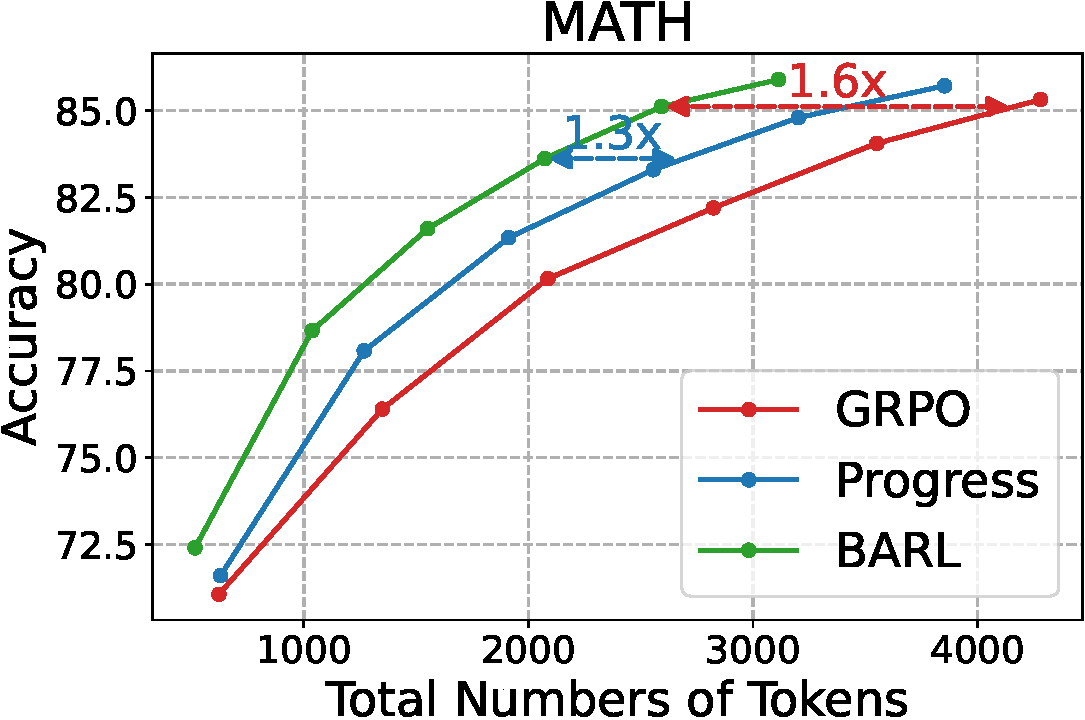
\includegraphics[width=1.033\linewidth]{figs/qwen15_math_token_2.pdf}
    \end{minipage}
    \begin{minipage}[b]{0.245\linewidth}
        \centering
        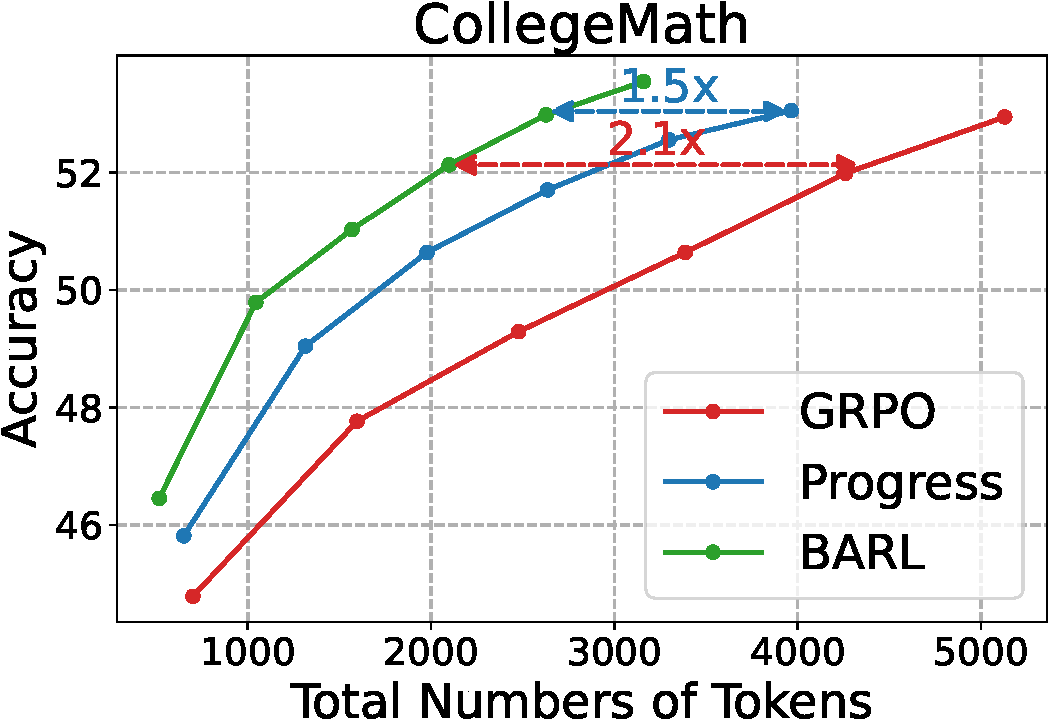
\includegraphics[width=\linewidth]{figs/qwen15_collegemath_token_2.pdf}
    \end{minipage}
        \begin{minipage}[b]{0.245\linewidth}
        \centering
    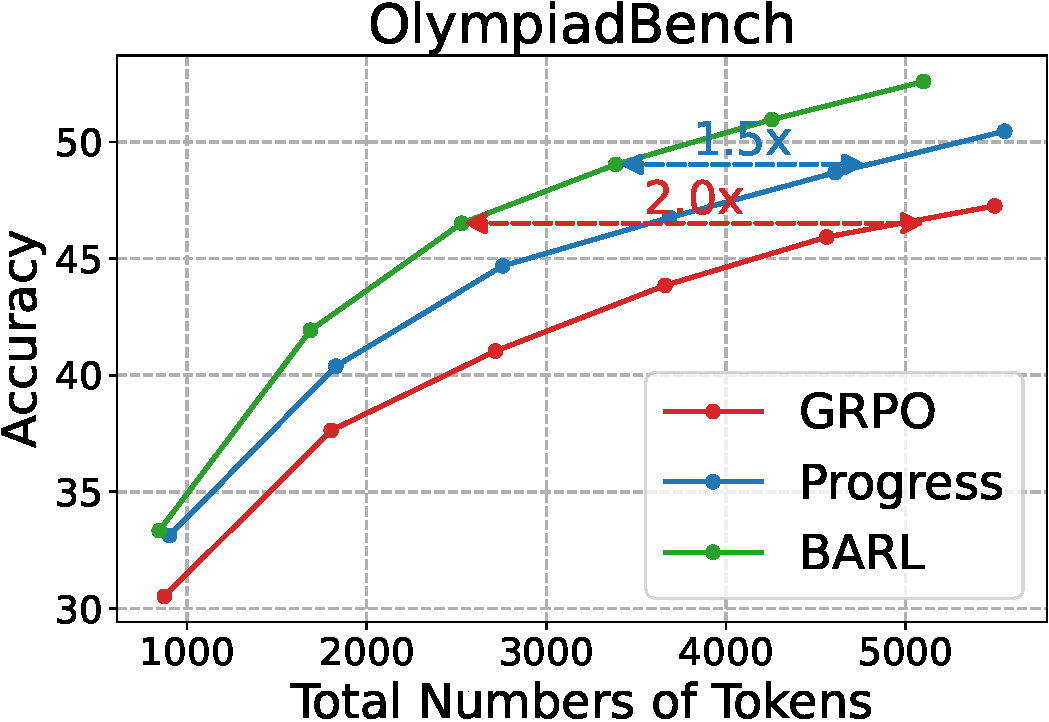
\includegraphics[width=\linewidth]{figs/qwen15_olym_token_2.pdf}
    \end{minipage}
\vspace{-0.5cm}
\setlength{\belowcaptionskip}{-15pt}
\caption{BARL is more token efficient, achieving higher accuracies with fewer total numbers of tokens.\vspace{-0.1cm}}
\label{fig_ablation_token}
\end{figure}

\begin{wrapfigure}{r}{0.283\textwidth}
     \vspace{-0.3cm}
    \begin{minipage}[t]{0.283\textwidth}
        \centering
        \begin{minipage}[t]{\linewidth}
            \centering
            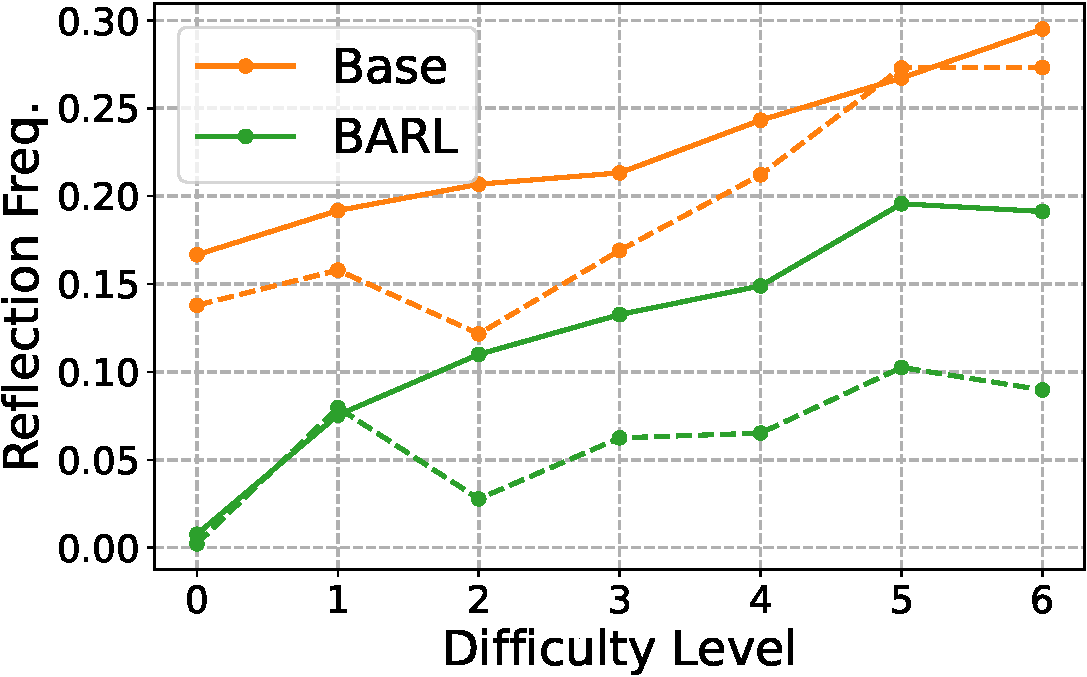
\includegraphics[width=\linewidth]{figs/qwen15_sr.pdf}
        \end{minipage}
        \vspace{-0.72cm}
        \setlength{\belowcaptionskip}{-10pt}
        \caption{Results on GSM8K (dashed) and MATH (solid).}
        \label{fig_sr}
    \end{minipage}
\end{wrapfigure} 

\vspace{-0.15cm}
\paragraph{Reflective Reasoning Behaviors.} To qualitatively assess the improved token efficiency of BARL, we analyze the frequency of reflective behaviors across problems of varying difficulty levels, as shown in Figure \ref{fig_sr}. For each problem,  we sample $6$ responses per model and define its difficulty level by the number of incorrect responses. We use keyword-based detections \citep{liu2025understanding,yeo2025demystifying} to identify whether self-reflections appear in a response, and a problem is considered to exhibit self-reflection if at least one of its responses is identified. It can be observed that both models display fewer reflections on easier problems, and the base model exhibits a higher frequency of reflections despite achieving lower accuracies. This result reveals (1) the base model has acquired superficial stylistic reflection patterns during pre-training (e.g., from CoT annealing data) without effective exploration, whereas BARL yields more effective reflective exploration rather than stylistic patterns; and (2) the weak correlation between the performance of LLMs and the response length or the frequency of reflections. Rather, the effectiveness of thinking tokens and the efficiency of explorations are the determining factors, which we study in the following ablation.

\vspace{-0.15cm}
\paragraph{Effectiveness of CoTs.} We measure the effectiveness of the CoTs produced by different models by calculating the average Bayesian state-action values at each timestep, which naturally captures both the exploration and the exploitation aspects of the actions. 
Specifically, the Bayesian value is defined as $Q^\pi(b_t, s_t, a_t) = \EE_{\pi, \mathcal{M}\sim b_t}[r_{\mathcal{M}}(s_t, a_t) + Q^\pi(b_{t+1}, s_{t+1}, a_{t+1})]$, where the belief $b_t=p(\mathcal{M}|h_t)$. 
Unlike standard Q-values, the Bayesian Q-value not only incorporates the expected returns (exploitation) but also captures the value of information gained through belief updates (exploration). 
\begin{figure}[h]
\vspace{-0.2cm}
    \centering
    \begin{minipage}[b]{0.245\linewidth}
        \centering
        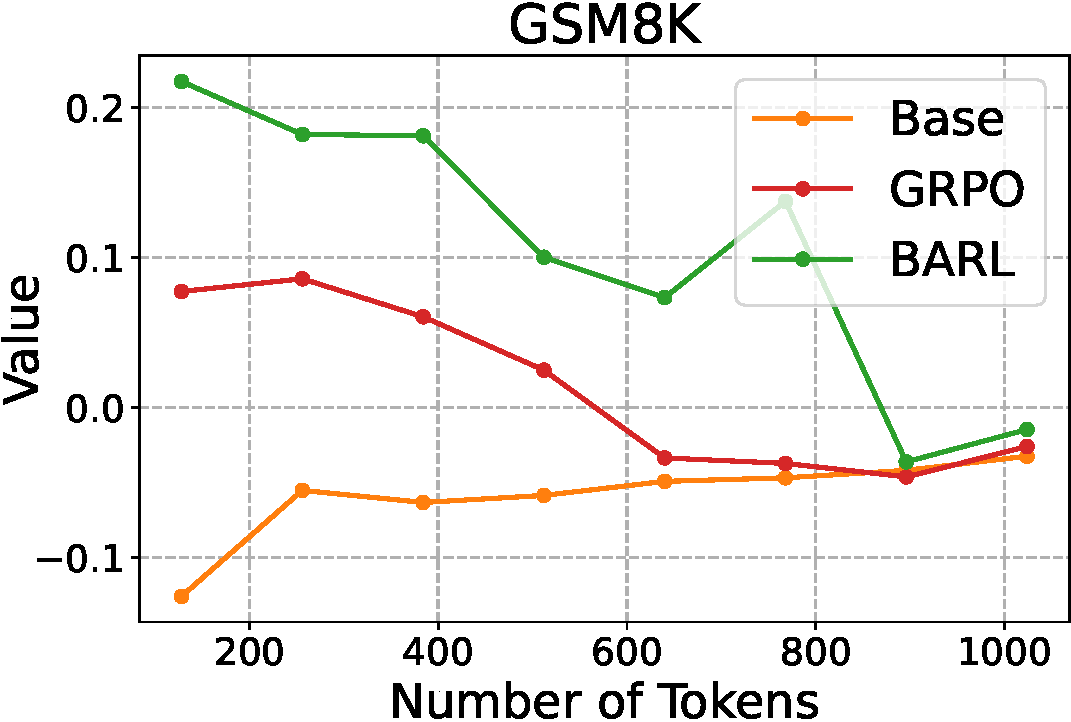
\includegraphics[width=0.98\linewidth]{figs/qwen15_gsm_q.pdf}
    \end{minipage}
    \begin{minipage}[b]{0.245\linewidth}
        \centering
        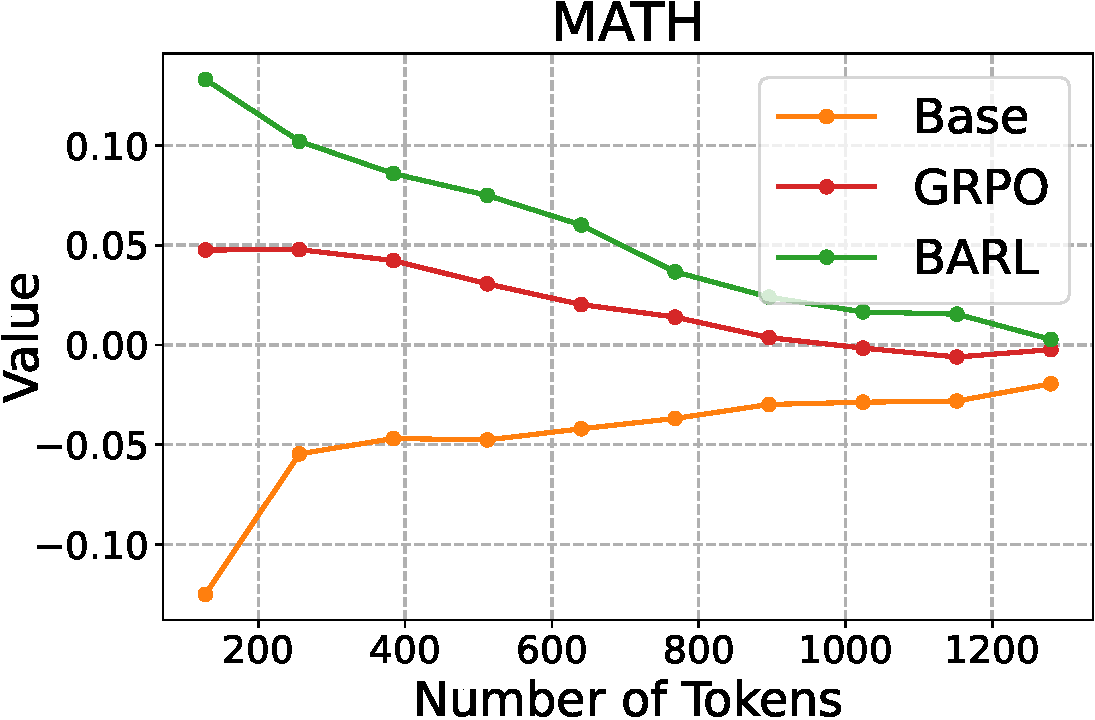
\includegraphics[width=\linewidth]{figs/qwen15_math_q.pdf}
    \end{minipage}
    \begin{minipage}[b]{0.245\linewidth}
        \centering
        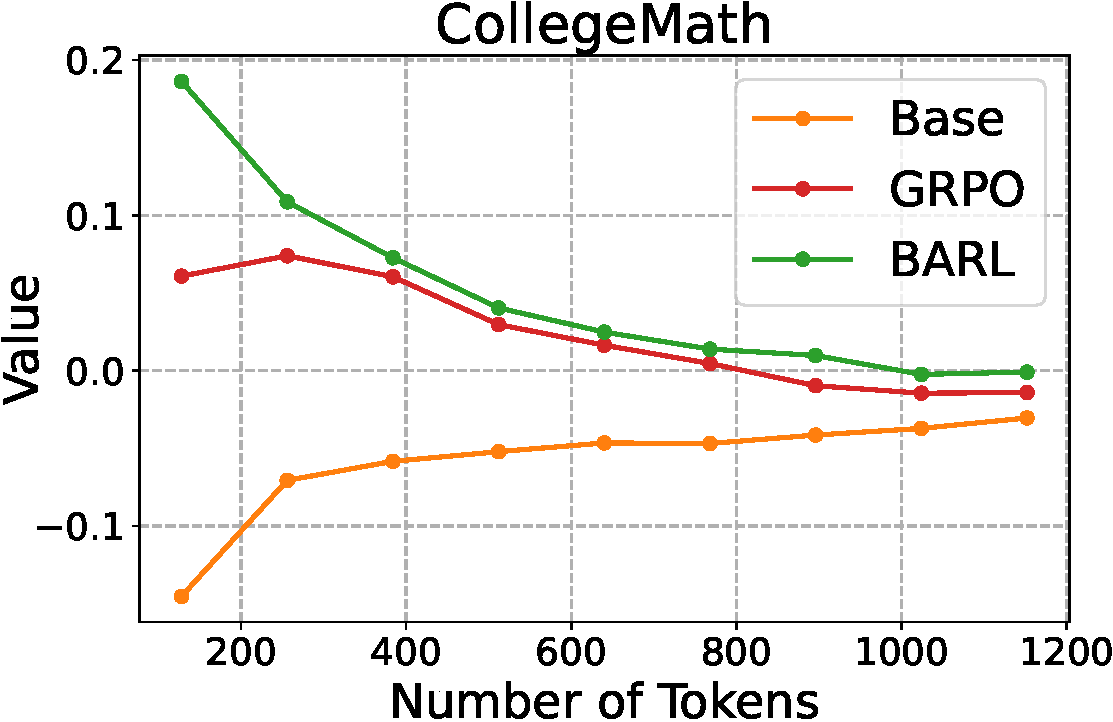
\includegraphics[width=1.018\linewidth]{figs/qwen15_collegemath_q.pdf}
    \end{minipage}
        \begin{minipage}[b]{0.245\linewidth}
        \centering
    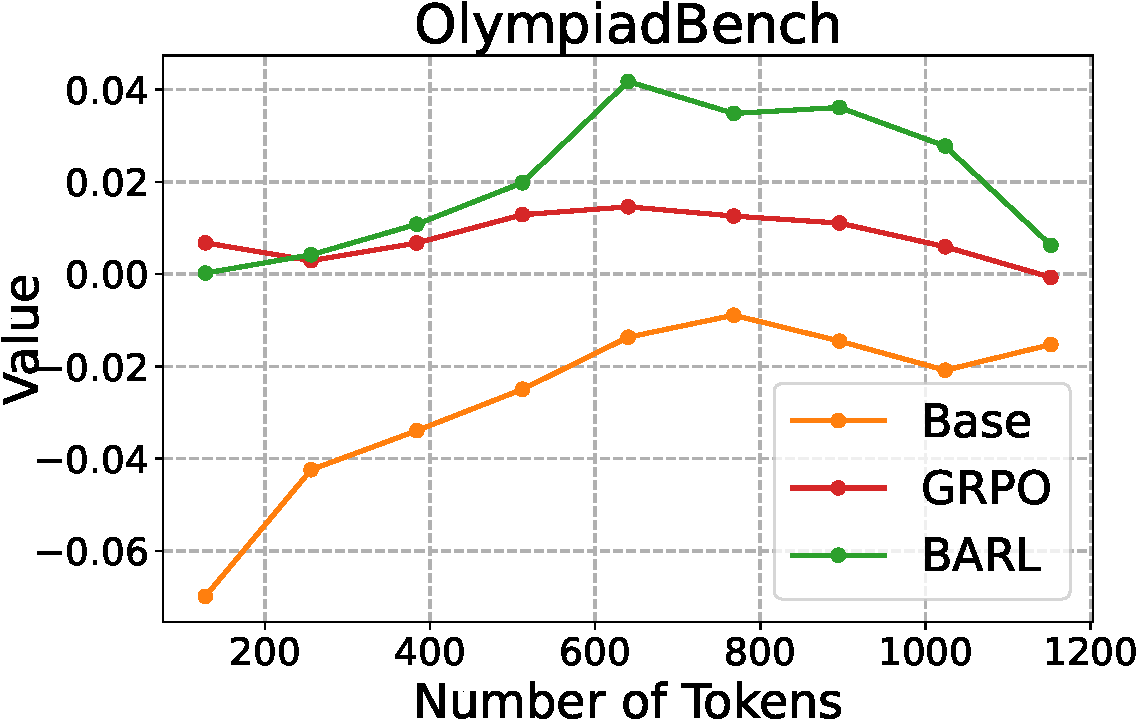
\includegraphics[width=1.038\linewidth]{figs/qwen15_olym_q.pdf}
    \end{minipage}
\vspace{-0.5cm}
\caption{Ablation on how effective the CoTs explore and exploit, measured by the Bayesian values. \vspace{-0.4cm}}
\label{fig_ablation_value}
\end{figure}

The results are reported in Figure \ref{fig_ablation_value}. We observe that the actions from the BARL model exhibit consistently higher Bayesian values compared to those of the GRPO and base models, indicating more effective exploration and exploitation. 
On more challenging benchmarks such as OlympiadBench, exploratory gains peak midway through the CoTs after an early phase of uncertainty reduction. Moreover, the result also explains our earlier observations on token efficiency and reflective behaviors. Although the base model exhibits more self-reflections, these are likely superficial or stylistic patterns due to their low exploration efficiency for gathering informative contexts during evaluation.

\vspace{-0.15cm}
\paragraph{Markovian RL Optimality.} We train a length-controlled (LC) GRPO with a maximum $32$ response length over multiple epochs. Figure \ref{fig_ablation_opt} shows the evolution of the training accuracy and length. The rapidly increasing accuracy and decreasing response length of GRPO LC indicate that it learns to skip CoT generation and emit only the final answer. Its asymptotic training accuracy matches that of GRPO (max length $1024$). This result supports Theorem \ref{remark_1}: Markovian RL can achieve optimality by merely memorizing solutions without reflective reasoning. Such policies, however, generalize poorly during evaluation. We refer readers to Appendix \ref{app_more_exp} for additional experimental results.

\begin{figure}[h]
\vspace{-0.1cm}
    \centering
    \begin{minipage}[b]{0.245\linewidth}
        \centering
        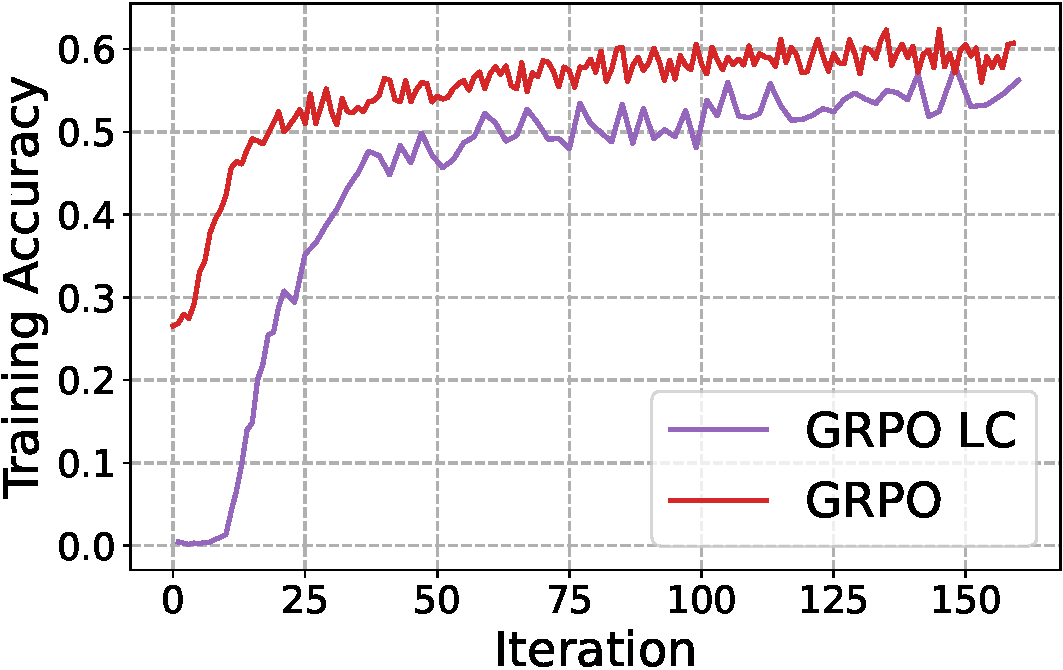
\includegraphics[width=\linewidth]{figs/grpo_lc_acc.pdf}
    \end{minipage}
    \hspace{0.35cm}
    \begin{minipage}[b]{0.245\linewidth}
        \centering
        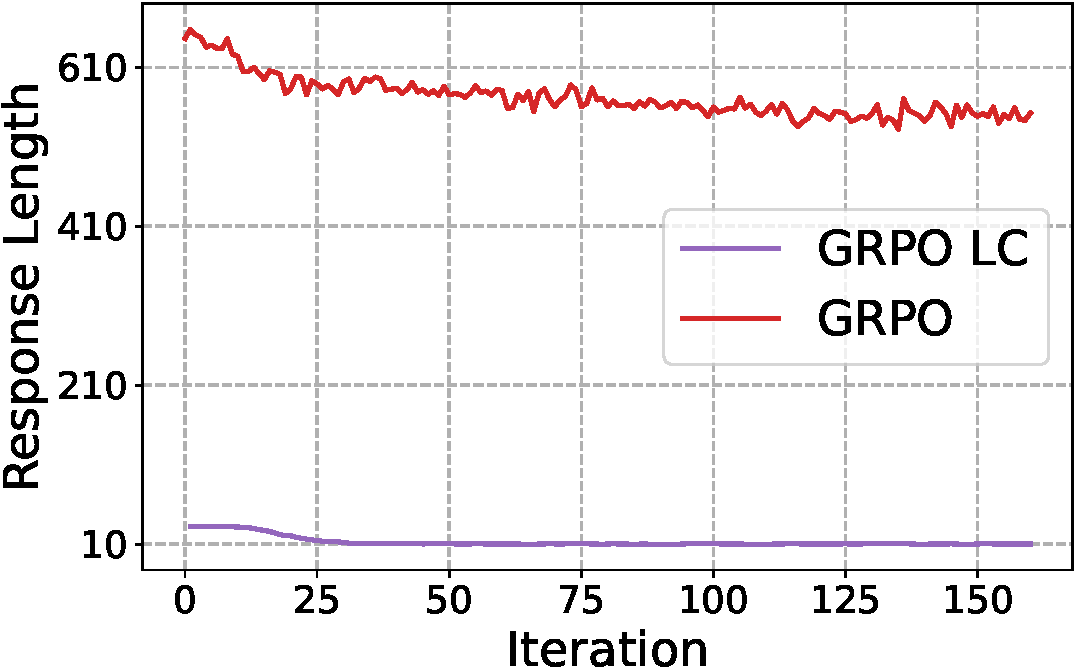
\includegraphics[width=1.013\linewidth]{figs/grpo_lc_len.pdf}
    \end{minipage}
        \hspace{0.35cm}
        \begin{minipage}[b]{0.245\linewidth}
        \centering
    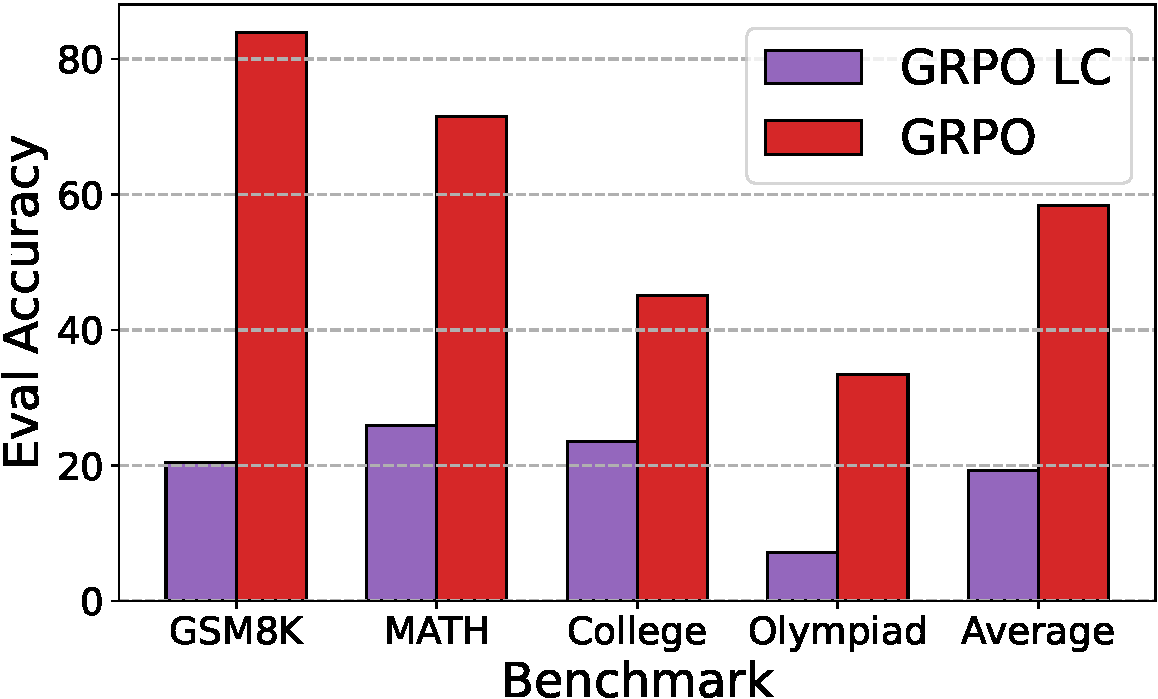
\includegraphics[width=1.048\linewidth]{figs/grpo_lc_eval.pdf}
    \end{minipage}
\vspace{-0.1cm}
\caption{\textbf{(Left)} Training accuracy. \textbf{(Middle)} Training response length. \textbf{(Right)} Final evaluation results.}
\label{fig_ablation_opt}
\end{figure}

\begin{AIbox}{\text{Key Experiment Findings}}
BARL consistently outperforms conventional RL baselines with superior token efficiency. Performance correlates with the effectiveness of reflective explorations, rather than their frequency. Optimality in conventional RL can be attained by policies that memorize training solutions yet fail to generalize, with no guarantees on the emergence of self-reflections.
\end{AIbox}